
% ----------------------------------------------
\chapter{Modelling Polarization}
\label{sec: ch5_DustScatteringModels}
% ----------------------------------------------



Modelling the dust polarization from scattering across multi-wavelength data allows us to constrain the dust grain size using a method adapted from \cite{Zhang2023}, which is detailed below. The geometric modelling of the observations in Chapter \ref{sec: methods/modelling polarization pattern} was used to identify the region of the disk at each wavelength where the observed polarization morphology aligned with the minor axis, consistent with dust self-scattering. This region provides a constraint for the dust grain size. The goal of the modelling is to model the dust properties in this region using spherical and irregular grains and compare the amount of polarized light to the observed polarization fraction of IRS 63 to constrain the dust grain size. Several parameters are used throughout the dust model calculations. Table \ref{tab:dust_parameters} summarizes these parameters for reference. 



% ----------------------------------------------
\begin{table}[ht]
\centering
\caption[Summary of parameters for dust scattering model calculations.]{Summary of parameters repeatedly used throughout the dust scattering model calculations. } 
\label{tab:dust_parameters}

\begin{tabular}{lll}
\toprule
\textbf{Symbol} & \textbf{Parameter} & \textbf{Units} \\
\midrule
$a_{\max}$  & Maximum dust grain size in distribution grid & $\mu$m \\
$\lambda$   & Observing wavelength & mm \\
\achar & Characteristic grain size  & $\mu$m \\
$\kappa_{\text{abs}}$, $\kappa_{\text{sca, eff}}$ & Mass absorption and effective scattering coefficients & cm$^2$/g\\
$\Theta$ & Scattering Angle & degrees \\
\weff & Effective single scattering albedo & -- \\
$P$  & Polarization fraction predicted from model at $\Theta$ = 90\degg & \% \\
\Pweff & Polarization from model & \% \\
$f$  & Filling factor & -- \\
\POLFsi & Polarization fraction at the pixel with maximum Stokes $I$ & \% \\
SF  & Scale factor & -- \\
$\chi^2_{\mathrm{P}}$ & Chi-squared statistic for the polarization fraction fit & -- \\
\bottomrule
\end{tabular}
\begin{tablenotes}
% \footnotesize
\item \textbf{Note:} $\lambda$ is reported in mm, while \achar and \amax are reported in \micronNS. For calculations involving $\lambda$ and \amaxNS, they are converted to cm for the calculations. 
\end{tablenotes}
\end{table}
% ----------------------------------------------





% ----------------------------------------------
\section{Model Assumptions}
\label{sec: model_assumptions}

% ----------------------------------------------

% ----------------------------------------------
\subsection{Grain Shape}
% ----------------------------------------------
Two grain geometries were explored: spherical grains and irregular grains. The model assumptions described in this chapter apply to both the spherical and irregular grain models. If there is a slight difference, it will be specified. 

Spherical dust grain modelling is a more common approach the scattering properties of spheres have simpler calculations. The scattering properties for spherical grains were calculated using the DSHARP Mie-Opacity Library (\texttt{DSHARP}) from \cite{dsharp_code}. 


Irregular grains were tested as they are a more realistic shape for dust grains in disks \citep{Lin2024}. The more complicated irregular grain shape affects the scattering properties, making the calculations more difficult and computationally expensive. However, these calculations have become more accessible with \texttt{glitterin} (dust Grain LIght scaTTERIng Neural network) from \cite{glitterin}. Figure \ref{fig: glitterin_dust_grains} shows an example of six irregular grain shapes from \texttt{glitterin}.


\begin{figure}[htbp]
  \centering
  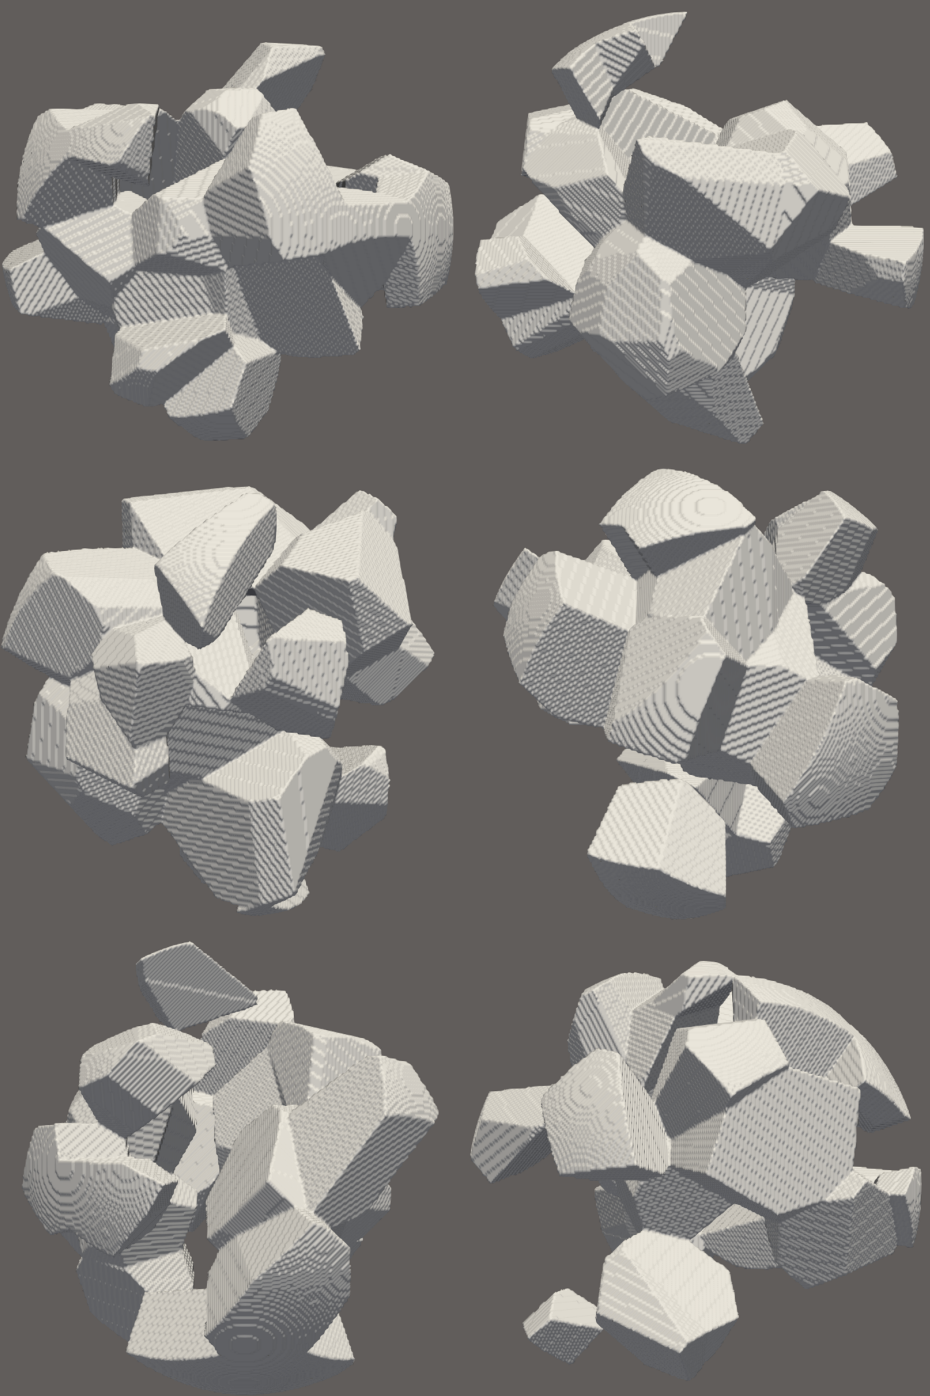
\includegraphics[width=0.3\textwidth]{WRITEUP_AND_IMAGES/IMAGES/WRITEUP/NOTMINE/glitterinFigure1.png}
  \caption[Example of six irregular particles from \texttt{glitterin}.]{Example of six irregular particles from \texttt{glitterin}. Figure from \cite{glitterin}. \permission{ask for permission} }
  \label{fig: glitterin_dust_grains}
\end{figure}
% ----------------------------------------------



% ----------------------------------------------
\subsection{Dust Composition}
% \label{sec: measured_POLF}
% ----------------------------------------------
The dust grains are assumed to follow the Disk Substructures at High Angular Resolution Project (DSHARP) dust composition, consisting of water ice, astronomical silicates, troilite and refractory organic material \citep{dsharp_code}. The corresponding volume fractions, mass fractions, bulk densities, and sources for the refractive indices are listed in Table \ref{tab: dsharp_composition}. 




\begin{table}[h!]
\centering
\caption{DSHARP dust composition used in this project.}

\begin{tabular}{lllll}
\toprule
\textbf{Material} &
\shortstack[l]{\textbf{Bulk Density}\\\textbf{(g cm$^{-3}$)}} &
\shortstack[l]{\textbf{Volume}\\\textbf{Fraction}} &
\shortstack[l]{\textbf{Mass}\\\textbf{Fraction}} &
\shortstack[l]{\textbf{References}} \\
\midrule
Water Ice
& 0.92
& 0.3642
& 0.2000
& (1) \\

Astronomical Silicates
& 3.30
& 0.1670
& 0.3290
& (2) \\

Troilite
& 4.83
& 0.02578
& 0.07434
& (3) \\

Organics
& 1.50
& 0.4430
& 0.3966
& (3) \\

\bottomrule
\end{tabular}
\begin{tablenotes}
% \footnotesize
\item \textbf{Note:} References for the refractive index are: (1) \cite{Warren_and_Brandt}, (2) \cite{Draine}, and (3) \cite{Henning_and_Stog}. DSHARP dust composition is from \cite{dsharp_code}
\end{tablenotes}
\label{tab: dsharp_composition}
\end{table}



% ----------------------------------------------
\subsection{Dust Size Distribution}
\label{sec: ch5_amax_distribution}
% ----------------------------------------------

The dust grains were assumed to have a size distribution of $n(a)\propto a^{3.5}$, chosen to match the distributions used by \cite{Kataoka_2015} and \cite{Zhang2023}. The minimum grain size is 0.1 \micronNS, while the maximum grain size is varied in logarithmic space up to 5000 \micronNS, with 2000 values sampled in total. The maximum grain size in each distribution is denoted by \amaxNS. For the irregular grain models, a lower limit of dust grain size of 2 \micron was used to avoid Nan values being produced in \texttt{glitterin}.


% ----------------------------------------------
\subsection{Porosity/Filling Factor and Density}
% ----------------------------------------------
Porosity ($p$) is the fraction of a dust grain's volume that is empty space. A low porosity corresponds to a more compact grain (like a rock), while a high porosity corresponds to a grain with more empty space (like a sponge). Instead of specifying the porosity directly, the filling factor ($f$) is used, defined as:
\begin{equation}
 f = 1 - p,
    \label{eq: filling factor}
\end{equation}
\noindent where $f=1$ corresponds to a compact grain ($p$ = 0), and an $f$ value less than 1 corresponds to a more porous grain \citep{Zhang2023}. 

The porosity cannot be varied for irregular dust grains, so only compact grains were tested. However, for spherical grains, a range of filling factors was tested ($f = 1, 0.75, 0.60, 0.5, 0.3, 0.25, 0.1, 0.01$) to sample different dust grain porosities. The results for $f = 1, 0.5, 0.3, 0.1$ are discussed in more detail, and some results for $f = 0.75, 0.25, 0.01$ are included. For each filling factor, the \texttt{DSHARP} code was used to calculate the corresponding density and optical constants of the dust mixture. Table \ref{tab:dsharp_density} lists  the resulting density values. As expected, the density decreases as the filling factor decreases and the porosity increases.  


% \noindent \question{Add more detail on how the \texttt{DSHARP} code incorperates different filling factors?} \SC{A: You haven't defined opacity yet.  You may want to wait until you get to equations that use the porosity.}

%\add{Question from disks on the exe: different function? How does the code integrate the different porosities}

\begin{table}[h!]
\centering
\caption{Summary densities calculated using \texttt{DSHARP} for each filling factor.}
\begin{tabular}{ll}
\toprule
\textbf{Filling Factor (\boldmath$f$)} &
\textbf{Density (g/cm\boldmath$^3$)} \\
\midrule
1.0    & 1.675 \\
0.5 & 0.838 \\
0.3  & 0.503 \\
0.1 & 0.168 \\
\bottomrule
\end{tabular}
\label{tab:dsharp_density}
\end{table}
% ----------------------------------------------



\subsection{Spherical Grain Geometry \& Mie Theory}
% \label{sec: ch5_mie_achar}


 
The size of a spherical dust grain is defined by its radius ($a$), with a corresponding size parameter ($x$) given by:
\begin{equation}
 x = \frac{2\pi a}{\lambda},
 \label{eq: size_parameter}
\end{equation}
\noindent where $\lambda$ is the observing wavelength \citep{Zhang2023}. When the size parameter is equal to 1, the corresponding grain size is defined as the characteristic grain size ($a_{\text{char}}$), given by $\lambda/2\pi$. As discussed in Chapter \ref{sec: intro_dust_grainsize}, this is the grain size at which dust self-scattering is most efficient. 


The size parameter controls the way the light interacts with the dust grains by determining the scattering regime of the dust grains (Mie theory) \citep{Zhang2023}:
\begin{enumerate}
    \item $x \ll 1$: Rayleigh regime,
    \item $x \sim 1$: Mie regime,
    \item $x \gg 1$: geometric regime.
\end{enumerate}

% ----------------------------------------------



% ----------------------------------------------
\subsection{Irregular Dust Grains \& \texttt{glitterin}}
\label{sec: ch5_glitterin}
% ----------------------------------------------
Rather than using Mie theory, which is for spherical grains, \texttt{glitterin} uses a neural network trained to predict light scattering from irregularly shaped dust grains. Predictions are made based on input parameters such as size parameter. 



Since irregular grains do not have a clear radius like spherical grains do, the \texttt{glitterin} code allows the user to choose between three options to define the size of the grain. First, \renc is the radius of the smallest sphere that can contain the irregular grain. Secondly, \rvol is the radius of a sphere with the same volume as the irregular grain. Third, \rpja is the radius of the sphere with the same projected geometric area as the irregular grain. In this project, we chose to use \rvol for our radius, or maximum grain size. Using this \rvolNS, the size parameter for the irregular grain can be calculated using Equation \ref{eq: size_parameter} such that:
\begin{equation}
    x_\text{vol} = \frac{2 \pi r_\text{vol}}{\lambda}.
\end{equation}
\noindent 
% ----------------------------------------------







% ----------------------------------------------
\subsection{Computing Optical Properties}


The complex refractive index ($m$) describes the optical properties of the dust and is given by:
\begin{equation}
 m(\lambda) = n(\lambda) + ik(\lambda),
\end{equation}
\noindent where $n$ and $k$ are the real and imaginary parts of the refractive index, respectively \citep{Zhang2023}. These values are calculated for each observing wavelength using \texttt{DSHARP}, and does not vary with porosity or grain shape. 


For spherical grains, at each filling factor and grain size in the distribution, \texttt{DSHARP} calculates several additional optical properties. \texttt{DSHARP} requires the user to specify the grain size, observing wavelength, and porosity. These additional optical properties calculated by the respective computational tools include the mass absorption and scattering coefficients, \kabs and \kscaNS, respectively. These coefficients describe how efficiently a material absorbs and scatters light. The resulting quantities are averaged over the grain-size distribution and are used to calculate additional parameters described below. 


The \texttt{glitterin} functions do not directly calculate \kabs and \ksca directly, but it calculates the absorption and scattering cross sections, $C_\text{abs}$ and $C_\text{sca}$. These can be used to calculate \kabs and \ksca given by:
\begin{equation}
    \kappa_i = \frac{C_i}{\frac{4\pi}{3}\rho_s r_\text{vol}^3},
\end{equation}
\noindent where $i$ can be abs or sca, and $\rho_s$ is the density from a compact grain with DSHARP dust composition. To calculate the $C_i$ values with \texttt{glitterin}, it requires the user to specify \xvolNS, $n$, and $k$ which were calculated using \texttt{DSHARP}, the observing wavelength, and scattering angle (defined below). 






% Single scattering tells us of all the interactions between radiation and dust, what fraction are scattering or absorbing?

% A grain can be scattered but its direction barely changes, but it still increases k_sca and then omega, despite not being re-directed anywhere

% g is a parameter of how strongly scattering prefers the forward direction: g = 0 (isotropic, equally liklely to scatter in any direction), g > 0 (prefers forward), etc 



Scattering can have a bias towards the forward direction, such that a significant amount of scattering does not noticeably change the direction of the incident light. Since \ksca accounts for all scattering events, this bias can lead to \ksca overestimating the contribution of scattering. This bias is corrected by using the asymmetry parameter, $g$, defined as the expectation value of $\cos\Theta$, where $\Theta$ is the angle between the incident and scattered directions (the scattering angle). The parameter $g$ is used to calculate an effective scattering opacity, given by \citep{dsharp_code, Tazaki, Zhang2023}:
\begin{equation}
    \kscaeffEQ = (1-g)\kscaEQ.
\end{equation}
\noindent An additional quantity that can be calculated for spherical and irregular grains is the effective single scattering albedo, which describes the fraction of the original light that is removed by scattering rather than absorption. This is given by the equation \citep{Zhang2023}: 
\begin{equation}
    \weffEQ = \frac{\kscaeffEQ}{\kabsEQ + \kscaeffEQ}.
    \label{eq: omega}
\end{equation}
 



Figure \ref{fig: Kataoka2015Figure1Recreation} shows the absorption and effective scattering mass opacities as a function of observing wavelength for maximum grain sizes of \amax = 1 \micron and 100 \micron for compact and porous grains. For small compact grains, the absorption opacity is much greater than the effective scattering opacity at wavelengths beyond $\sim$0.003 mm. For larger compact grains, the effective scattering opacity is greater than the absorption opacity between wavelengths of $\sim$0.25--2.5 mm. The results for porous grains remain relatively similar, with the range in which scattering dominates for larger grains extending to $\lambda\sim$0.15-2.5 mm. This indicates that porosity does not greatly affect the overall mass opacities. The blue shaded region highlights the range of observing wavelengths considered in this project (\bseven to \bfourNS), and within these boxes the effective scattering opacity is greater than the absorption opacity for both compact and porous grains. However, for the larger grains, the absorption and scattering opacities begin to converge at longer wavelengths. Overall, Figure \ref{fig: Kataoka2015Figure1Recreation} similarity indicates that within the considered observing wavelengths, scattering is more efficient at shorter wavelengths, and the contribution from absorption becomes more important toward longer wavelengths.



% ----------------------------------------------
\begin{figure}[htbp]
  \centering
  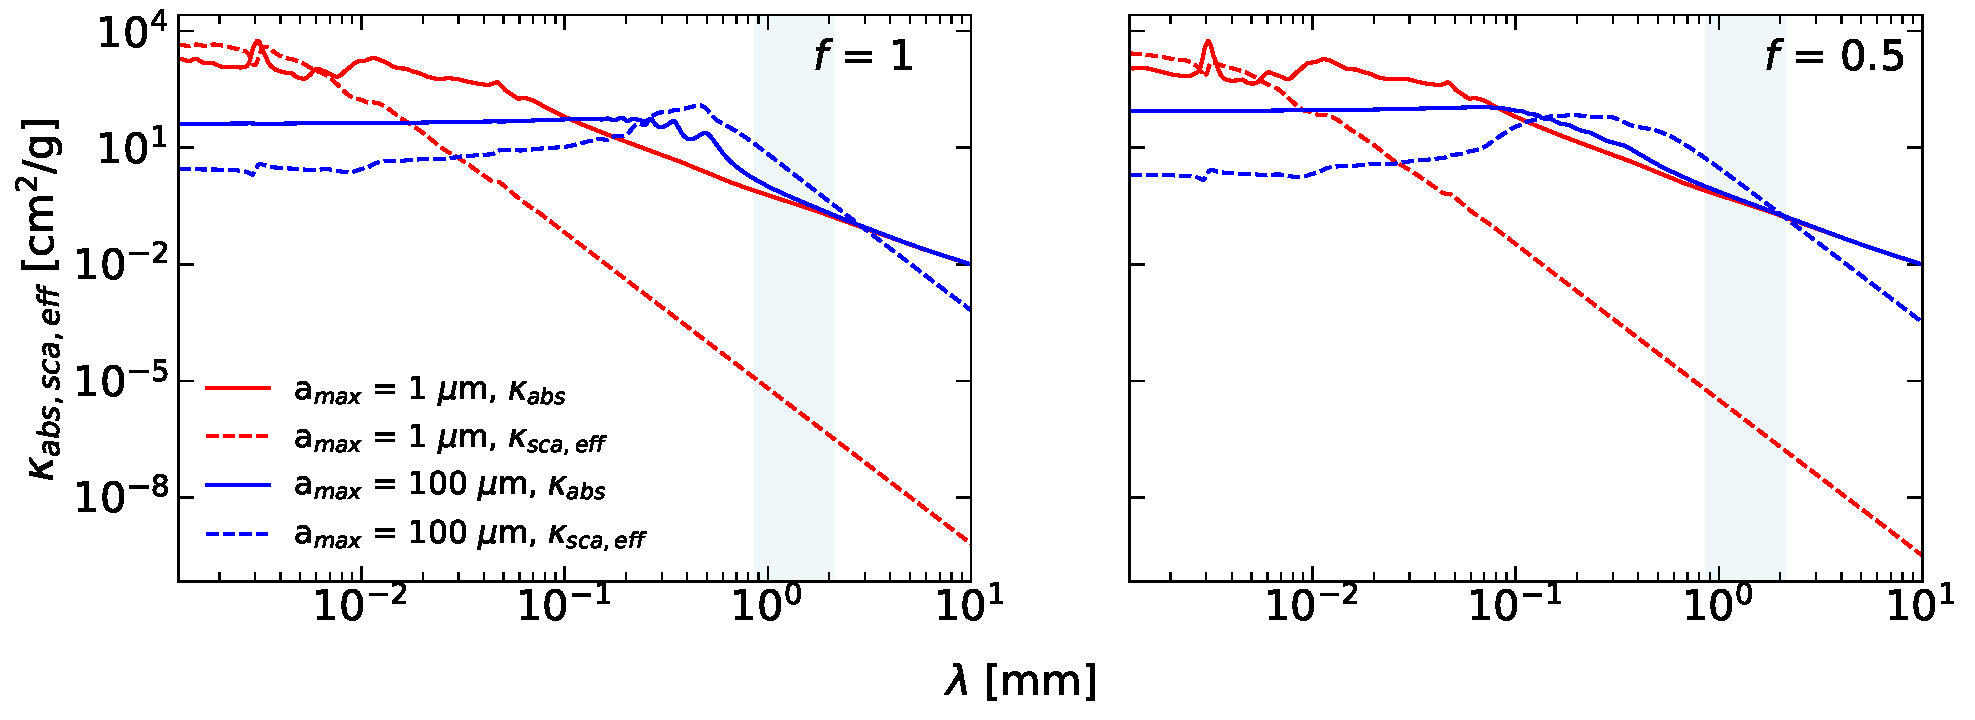
\includegraphics[width=0.99\textwidth]{WRITEUP_AND_IMAGES/IMAGES/WRITEUP/DustModels/Kataoka2015Fig1_grid_eff.pdf}
  \caption[Absorption and effective scattering mass opacities.]{Absorption and effective scattering mass opacities as a function of observing wavelength for grain sizes of 1\micron and 100 \micron for compact (left) and porous (right) grains. Blue box corresponds to lower limit of \bseven and upper limit of \bfourNS.}
  \label{fig: Kataoka2015Figure1Recreation}
\end{figure}
% Recreation of Figure 1 from \cite{Kataoka_2015}. 
% ----------------------------------------------

% ----------------------------------------------







% ----------------------------------------------
\subsection{Computing Polarization}
% ----------------------------------------------



The Mueller matrix, or scattering matrix, describes the polarization properties of light scattered by the dust grains \citep{Kataoka_2015} and is calculated using \texttt{DSHARP}. Two relevant matrix elements are \Zoo and \ZootNS, which represent linear polarized scattering and total scattering, respectively \citep{Zhang2023}. The polarization fraction is given by the ratio $-Z_{12, \text{eff}}/Z_{11, \text{eff}}$ averaged over the grain size distribution \citep{Kataoka_2015}. Figure \ref{fig: Kataoka2015Figure2Recreation} shows the dependence of polarization fraction on scattering angle for different maximum grain sizes. For smaller dust grains (10 \micron and 100 \micronNS), the polarization fraction peaks near a scattering angle of 90\deggNS. For larger dust grains (1 mm and 1 cm), the polarization fraction remains much closer to zero, indicating that polarization from scattering is not efficient for larger grains. In this analysis, the polarization fraction at 90\degg is denoted by $P$, and will be referred to as the polarization fraction. 









\begin{figure}[htbp]
  \centering
  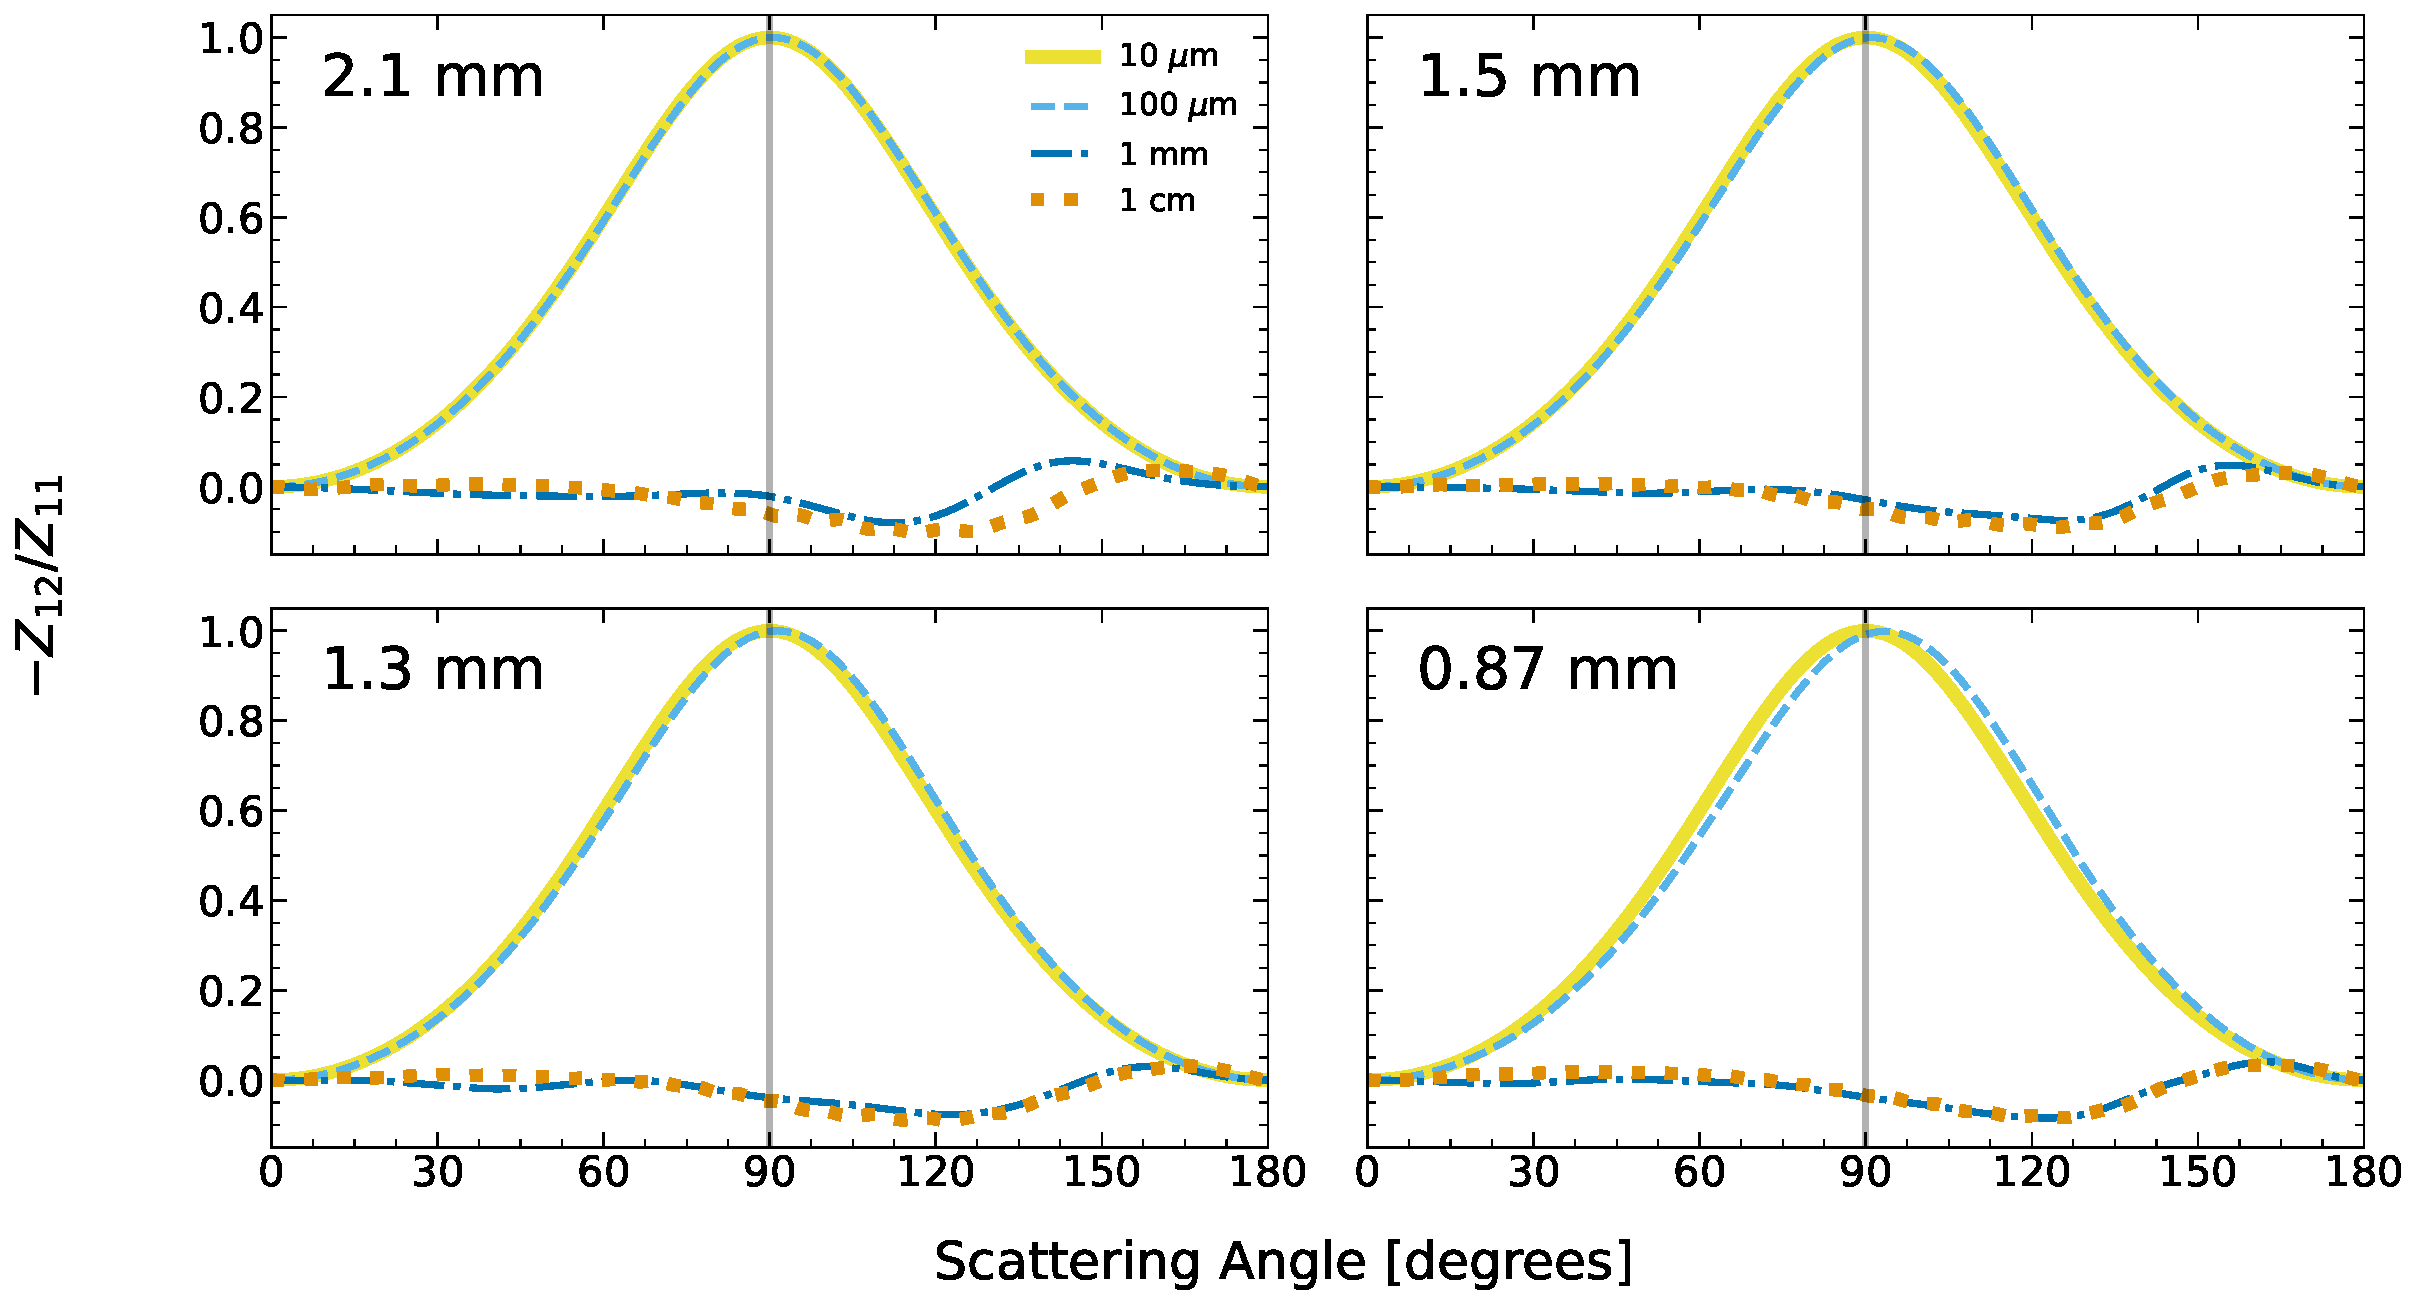
\includegraphics[width=0.99\textwidth]{WRITEUP_AND_IMAGES/IMAGES/WRITEUP/DustModels/Kataoka2015Fig2_grid.pdf}
  \caption[Polarization fraction as a function of scattering angle.]{Polarization fraction as a function of scattering angle for maximum grain sizes of 10 \micronNS, 100 \micronNS, 1 mm and 1 cm for compact dust grains. This is a replication of Figure 2 from \cite{Kataoka_2015}.}
  \label{fig: Kataoka2015Figure2Recreation}
\end{figure}

% ----------------------------------------------




% ----------------------------------------------
% \subsubsection{Polarization and Albedo as a Function of Grain Size}
% \label{sec: c5_P_and_w_vs_a}









% ----------------------------------------------
Figure \ref{fig: Kataoka2015Figure3Recreation} shows the polarization fraction and effective albedo as a function of maximum grain size for both compact and porous grains. For compact grains, it can be seen that the polarization fraction is larger for smaller grains and quickly decreases as the grain size increases above the observing wavelength.  . Conversely, the effective albedo increases with grain size, as larger grains have a larger surface area for the light to scatter off of. These curves (red and blue) have a distinctive peak, showing where the balance between polarization and scattering is most efficient. This peak is highlighted by plotting the product of the polarization fraction and the effective single-scattering albedo, \PweffNS, as a black dashed line. 

The \Pweff product provides a measure of the contribution of each grain size to the polarized scattered light at a specific observing wavelength, and can therefore be used to determine the grain sizes that contribute most strongly to the observed polarization \citep{Kataoka_2015, Tazaki}. As mentioned earlier, \achar is the grain size at which dust self-scattering is most efficient, so \Pweff is expected to peak near the characteristic grain size. This is shown as a grey line in each plot. For compact grains, the \Pweff peak occurs near \acharNS, as expected, highlighting the dependence of the polarization scattering efficiency on observing wavelength.

For porous grains (right panels of Figure \ref{fig: Kataoka2015Figure3Recreation}), the overall wavelength-dependent behaviour of the polarization and effective albedo remains similar, but their dependence on grain size is wider. The grain size at which the polarization fraction decreases and effective albedo increases is shifted toward larger grain sizes, causing the \Pweff curve to peak at a larger grain size than \acharNS. Additionally, the \Pweff peak is wider than the sharp peaks for compact grains. Together, these differences indicate that porous grains can efficiently contribute to polarized scattering at larger grain sizes and over a wider range of grain sizes compared to compact grains. This behaviour is assumed to be related to different scattering properties of porous grains due to their lower density and more empty space within the grains. 




\begin{figure}[htbp]
  \centering
  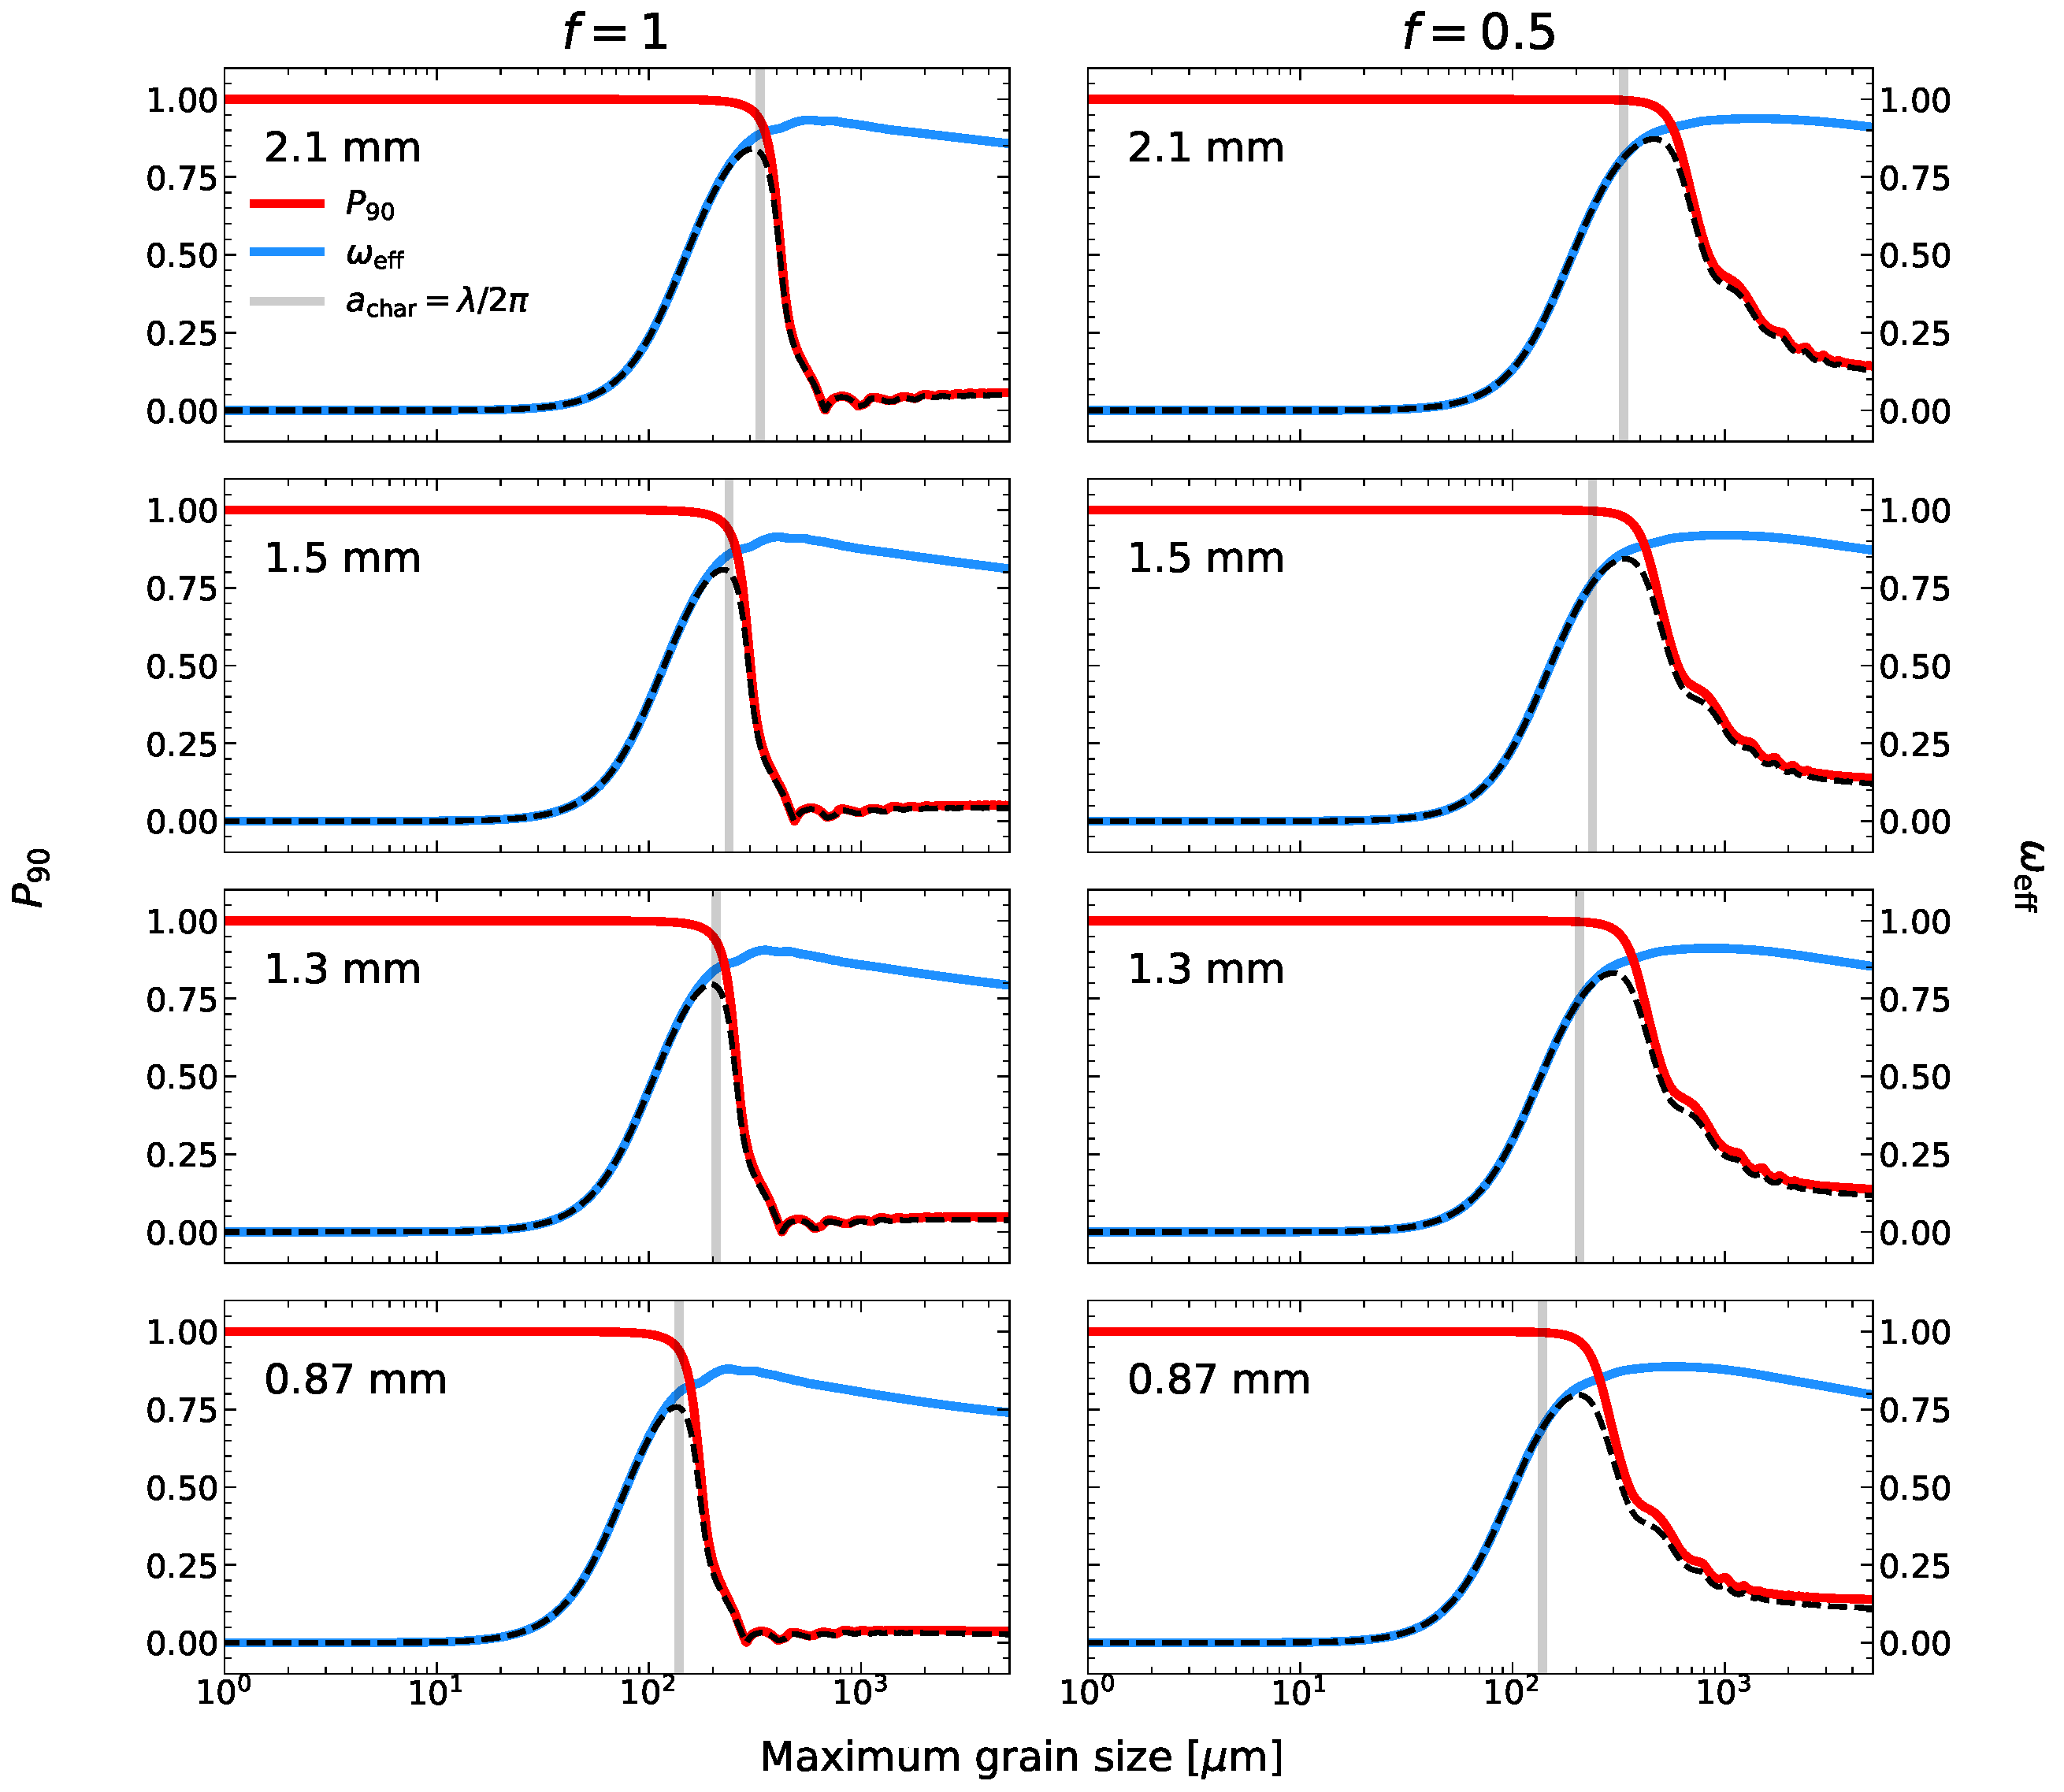
\includegraphics[width=0.99\textwidth]{WRITEUP_AND_IMAGES/IMAGES/WRITEUP/DustModels/P_vs_w_eff_vs_grainsize_grid_smooth_porosities.pdf}
  \caption[Polarization fraction $P$ and effective albedo as a function of grain size.]{Plot of polarization fraction $P$ in red and effective albedo in blue as a function of grain size for compact (left) and porous (right) dust grains. The characteristic grain size for each wavelength is over-plotted in grey, highlighting that it roughly corresponds to the local maxima of both curves. \question{Make this plot for irregular grains as well? If so, make it a separate plot or 3 columns?}}
  \label{fig: Kataoka2015Figure3Recreation}
\end{figure}

% ----------------------------------------------





Figure \ref{fig:Pweff_vs_grainsize} shows the \Pweff curves for compact spherical and irregular grains as a function of maximum grain size, with the characteristic grain size plotted as well for comparison. An additional plot for porous spherical grains can be seen in Figure \ref{fig: Pweff_vs_amax_porous}. While the behaviour of $P$ and \weff and their contributions to \Pweff are shown in Figure \ref{fig: Kataoka2015Figure3Recreation}, these plots highlight the importance of multi-wavelength data. The \Pweff curves generally peak near \acharNS, although as shown previously, the exact peak depends on porosity as well. More importantly, the peak \Pweff depends on grain size and observing wavelength, meaning that each wavelength is most sensitive to a different grain size. For the wavelengths considered in this project, the peaks occur at grain sizes of approximately hundreds of microns (Table \ref{tab: amax_peak_values}), indicating that polarization observations are most sensitive to grains in this range. By combining observations at multiple wavelengths, the grain size dependence can be utilized to provide a stronger constraint on the maximum grain size. The goal of this chapter is therefore to utilize the wavelength and grain size dependence of polarized scattering to determine the maximum grain size, shape, and porosity that best reproduces the observations. How the models are compared with the multi-wavelength observations is described in Chapter \ref{sec: ch5_determining_abest}.






% ------------------------------------------------------
\begin{table}[h!]
\centering
\caption[Maximum grain size corresponding to the peak \Pweff values. ]{Maximum grain size corresponding to the peak \Pweff values and characteristic grain size. }
\label{tab: amax_peak_values}
\begin{tabular}{lcccc}
\toprule
\textbf{Grain Size ($\boldsymbol{\mu}$m)} & \textbf{\bfour} & \textbf{\bfive} & \textbf{\bsix} & \textbf{\bseven} \\
\midrule

$a_{\text{char}}$
& 334.23
& 238.73
& 206.90
& 138.46 \\

$a_{\max}$ (spherical, compact)
& 307.88
& 223.71
& 196.46
& 134.50 \\


$a_{\max}$ (spherical, porous)
& 464.55
& 339.38
& 298.04
& 204.05 \\


$a_{\max}$ (irregular)
& 330.59
& 238.90
& 211.60
& 145.32 \\



\bottomrule
\end{tabular}
% \begin{tablenotes}
% \item \textbf{Note:} Corresponding figures for \Pweff curves are Figure \ref{fig:Pweff_vs_grainsize} for compact spherical and irregular, and Figure \ref{fig: Pweff_vs_amax_porous} for porous spherical. \achar can be seen in all three figures. 
% \end{tablenotes}
\label{tab: amax_peak_values}
\end{table}
% ------------------------------------------------------





% ----------------------------------------------
\begin{figure}[htbp]
  \centering

  \begin{minipage}[t]{0.48\textwidth}
    \centering
    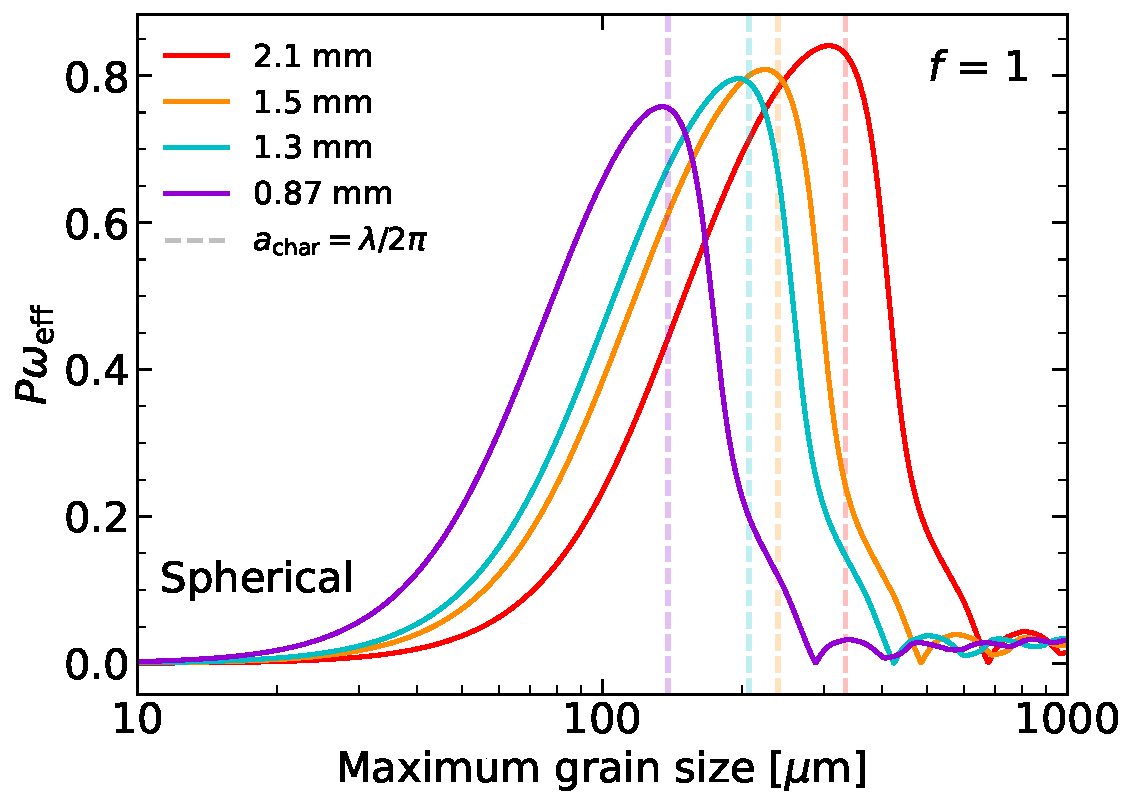
\includegraphics[width=\textwidth]{WRITEUP_AND_IMAGES/IMAGES/WRITEUP/DustModels/Pw_eff_vs_grainsize_compact.pdf}
  \end{minipage}
  \hfill
  \begin{minipage}[t]{0.48\textwidth}
    \centering
    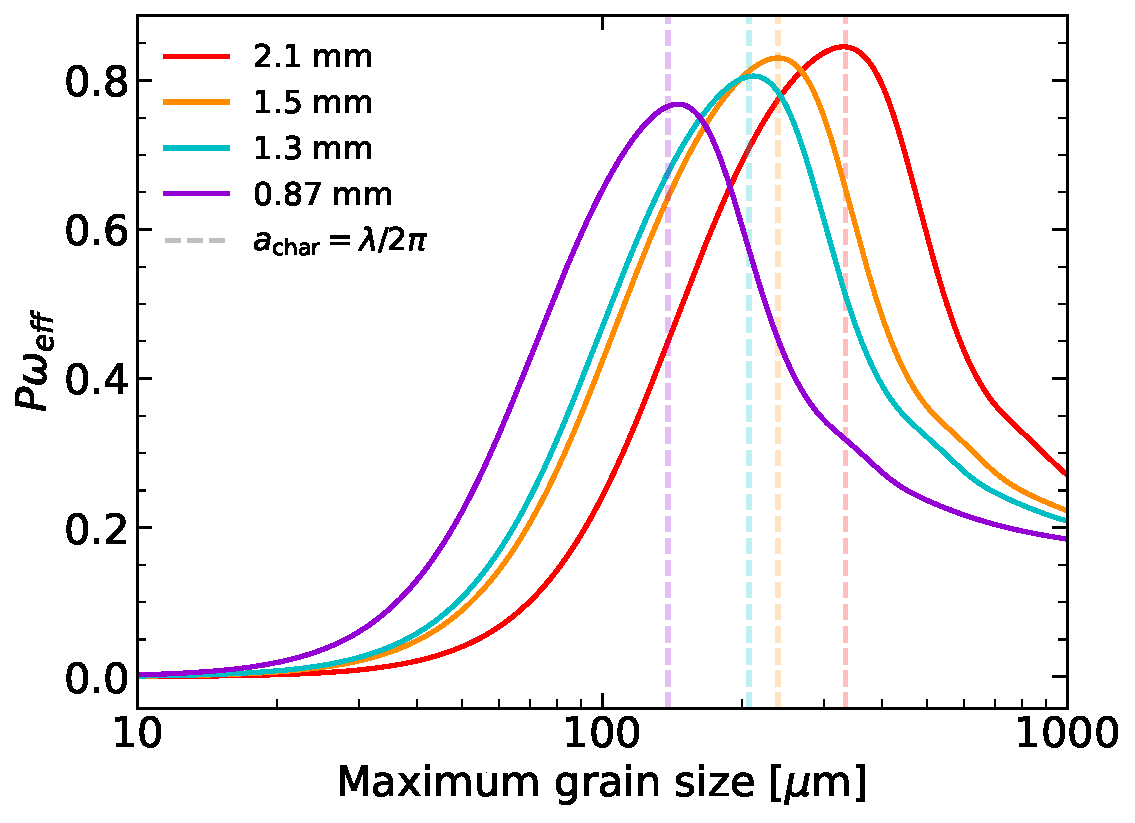
\includegraphics[width=\textwidth]{WRITEUP_AND_IMAGES/IMAGES/WRITEUP/glitterin/Pw_eff_vs_grainsize.pdf}
  \end{minipage}
  \caption[\Pweff versus maximum grain size.]{Polarization curves (\PweffNS) versus maximum grain size for each wavelength for compact spherical grains (left) and irregular grains (right). Overplotted as a dashed line with matching colour is the characteristic grain size. }
  \label{fig:Pweff_vs_grainsize}
\end{figure}
% ----------------------------------------------




% ----------------------------------------------






%
%
%











% ----------------------------------------------


% ----------------------------------------------
\section{Measuring Observed Polarization Fraction \& Determining the Best-Fit Scale Factor}
\label{sec: ch5_determining_abest}
% ----------------------------------------------
% ----------------------------------------------
\subsection{Measuring Observed Polarization Fraction}
\label{sec: measured_POLF}
% ----------------------------------------------
The polarization fraction was selected from the region showing evidence of self-scattering (uniform minor axis alignment). Three methods were tested to determine the most appropriate polarization fraction for this region:
\begin{enumerate}
    \item \POLFsiNS: The polarization fraction at the pixel with maximum \SIns.
    \item $\mathcal{P}_{\mathrm{F, max\,\POLIeq}}$: The polarization fraction at the pixel with maximum polarized intensity.
    \item  $\mathcal{P}_{\mathrm{F, Gaussian}}$: The mean polarization fraction within the uniform region of the Gaussian model, defined as the region where $W_{\text{uniform}}$ is within 1\% of the peak value of 1.
\end{enumerate}
\noindent 

\noindent Table \ref{tab: polf_comparison} summaries the values from these three methods at each wavelength. $\mathcal{P}_{\mathrm{F, max\,\POLIeq}}$ has a slight bias due to the forward scattering bias observed in Chapter \ref{sec: ch4_intensity_profiles}. $\mathcal{P}_{\mathrm{F, Gaussian}}$ produces similar results at higher porosities, but the goodness-of-fit significantly drops at lower porosities, potentially because the polarized fraction does not follow the wavelength-dependent trend observed in the other two methods. Therefore, \POLFsi is the best representation of the polarization fraction per wavelength, and is used throughout the rest of the analysis. 

% This selected value is referred to as the observed polarization fraction and is denoted by \POLFobsNS. Note that the polarization fractions used here are referred to as observed to distinguish them from the model, but they are debiased. 




% ----------------------------------------------
% ----------------------------------------------
\begin{table}[h!]
\centering
\caption[Polarization fraction values in the region of observed dust self-scattering.]{Polarization fraction values from various methods tested in the region of observed dust self-scattering.}
\label{tab:polf_comparison}
\begin{tabular}{lllll}
\toprule
\textbf{Parameter} & \textbf{\bfour} & \textbf{\bfive} & \textbf{\bsix} & \textbf{\bseven} \\
\midrule

$\mathcal{P}_{\mathrm{F, max\,I}}$
& 1.37
& 1.40
& 1.46
& 1.04 \\

$\mathcal{P}_{\mathrm{F, max\,POLI}}$
& 1.56
& 1.51
& 1.49
& 1.08 \\


$\mathcal{P}_{\mathrm{F, Gaussian}}$
& 1.16
& 1.35
& 1.41
& 0.90 \\

\bottomrule
\end{tabular}
\label{tab: polf_comparison}
\end{table}
% ----------------------------------------------
% ----------------------------------------------



% ----------------------------------------------


% ----------------------------------------------
\subsection{Determining the Best-Fit Scale Factor}
% ----------------------------------------------
The polarization fraction (\POLFsiNS) and the \Pw model values from spherical and irregular grains cannot be directly compared because they represent different quantities. The observed polarization fraction is a dimensionless ratio of polarized intensity to total intensity, while \Pw is the polarization scattering efficiency of the dust. A scale factor (SF) is therefore introduced to relate the model values to observations. 


The scale factor is calculated at each \amax in the sample, given by:
\begin{equation}
\sfeq_i(\amaxEQ) = \frac{\POLFsiEQ(\amaxEQ)}{\PwEQ(\amaxEQ)},
    \label{eq: sf}
\end{equation}


\noindent where $i$ denotes each wavelength included in the fit. This provides a scale factor for each fitted wavelength at every value of \amaxNS. If a given grain size provides a good reproduction of the observations across all fitted wavelengths, the resulting scale factors should be similar between the wavelengths. For each value of \amaxNS, the standard deviation of the scale factors is calculated to determine the spread of the scale factors between wavelengths using \texttt{numpy.std}. 



The best-fit grain size (\amaxbestNS) is defined as the value of \amax where the standard deviation of the scale factors is minimized. The corresponding scale factor is the best-fit scale factor (\sfbestNS). The model \Pw values are multiplied by the \sfbestNS, allowing the model and observations to be directly compared.


Multiple wavelength combinations were tested to determine the effect of each wavelength of data on the success of the fit. The fits were (1) all wavelengths, (2) no \bfiveNS, and (3) just \bfour and \bsevenNS. Case (2) was tested due to issues with the \bfive data, explored in Chapter \ref{sec: discussion_band5_data_issues}.  A chi-squared value was calculated at each fitting case to determine the agreement between the model and observations, given by: 
\begin{equation}
\chi_\mathcal{P}^2 = \sum_{all\text{ }wavelengths} \left(\frac{\POLFobsEQ- [\Pweq (\amaxbestEQ) \times \sfbestEQ]}{\POLFerrEQ}\right)^2.
    \label{eq: chi_squared_dust_model}
\end{equation}
\noindent The calculation is summed over all wavelengths as each wavelength was included in the $\chi_\mathcal{P}^2$ calculation, regardless of whether it was included in the fit for the scale factor value or not. The fitting combination (e.g., each porosity or irregular dust model) that produced the lowest $\chi_\mathcal{P}$ value were chosen to be the best-fit model.
% ----------------------------------------------
% ----------------------------------------------







% ----------------------------------------------
\section{Results from Dust Scattering Models}
\label{sec: ch5_DustModelResults}
% ----------------------------------------------
\subsection{Spherical Dust Models}
\label{sec: chapter5_spherical_dust_model_results}
% ----------------------------------------------
Table \ref{tab: dust_model_fits_spherical} reports the results of the spherical dust models. For each fitting case, the best-fit scale factor from Equation \ref{eq: sf}, the corresponding $\chi_\mathcal{P}^2$ value (Equation \ref{eq: chi_squared_dust_model}), and the best-fit grain size (\amax corresponding to the best SF) are reported. The best fit for each fitting case is shown in bold. Figure \ref{fig: Spherical_BEST} shows the best overall fitting case, which excludes \bfiveNS. Equivalent plots for the other fitting cases are provided in Appendix \ref{chap: Appendix_DustModels}. The observed polarization fraction, \POLFsiNS, is shown as a colour-matched marker for each wavelength. 


These results show that, for all fitting cases, compact grains ($f = 1.0$) and very porous grains ($f = 0.01$) produced a significantly worse match to the models compared to the intermediate porosities. The goodness-of-fit improves at these intermediate filling factor values, reaching a minimum at $f = 0.5$, as shown in Figure \ref{fig: chi_vs_f}. 




\begin{table}[h!]
\centering
\caption[Spherical dust grain model fitting results.]{Spherical dust grain model fitting results, including the scale factor $\chi_\mathcal{P}^2$, and best-fit grain size. The best fit for each fit case is shown in bold text. \reduced{update this after reduced chi squared}}
\begin{tabular}{lcccc}
\toprule
\textbf{Fit Case} & \textbf{Porosity ($\boldsymbol{f}$)} & \textbf{Scale Factor (SF)} & $\boldsymbol{\chi_\mathcal{P}^2}$ & \textbf{$\boldsymbol{\amaxEQ}$ ($\boldsymbol{\mu}$m)} \\
\midrule

All wavelengths
& 1.00 & 2.24 & 28.80 & 162 \\
& 0.75 & 2.11 & 7.03 & 200 \\
& 0.60 & 2.10 & 2.46 & 225 \\
& \textbf{0.50} & \textbf{2.13} & \textbf{1.37} & \textbf{244} \\
& 0.30 & 2.26 & 2.67 & 287 \\
& 0.25 & 2.33 & 3.17 & 301 \\
& 0.10 & 2.95 & 6.32 & 360 \\
& 0.01 & 9.40 & 37.55 & 512 \\

\midrule

No \bfive 
& 1.00 & 2.38 & 34.30 & 163 \\
& 0.75 & 2.20 & 11.24 & 202 \\
& 0.60 & 2.16 & 3.79 & 202 \\
& \textbf{0.50} & \textbf{2.15} & \textbf{1.32} & \textbf{245} \\
& 0.30 & 2.27 & 2.19 & 290 \\
& 0.25 & 2.34 & 3.08 & 303 \\
& 0.10 & 2.97 & 5.56 & 362 \\
& 0.01 & 9.39 & 38.02 & 509 \\

% \midrule

% No \bsix
% & 1.00 & 2.38 & 34.03 & 163 \\
% & \textbf{0.50} & \textbf{2.13} & \textbf{1.35}  & \textbf{244} \\
% & 0.30 & 2.26 & 2.57  & 289 \\
% & 0.10 & 2.94 & 6.70 & 364 \\

\midrule

Just \bfour 
& 1.00      & 2.49 & 70.00  & 164 \\
and \bseven & 0.75 & 2.21     & 13.29 & 202 \\
& 0.60 & 2.16 & 3.91 & 227 \\
& \textbf{0.50} & \textbf{2.15} & \textbf{1.49} & \textbf{245} \\
& 0.30      & 2.27 & 2.43   & 290 \\
& 0.25      & 2.34 & 3.13   & 303 \\
& 0.10      & 2.95 & 6.63   & 366 \\
& 0.01      & 8.94 & 44.34  & 535 \\

\bottomrule
\end{tabular}
\label{tab: dust_model_fits_spherical}
\end{table}






\begin{figure}[htbp]
  \centering
  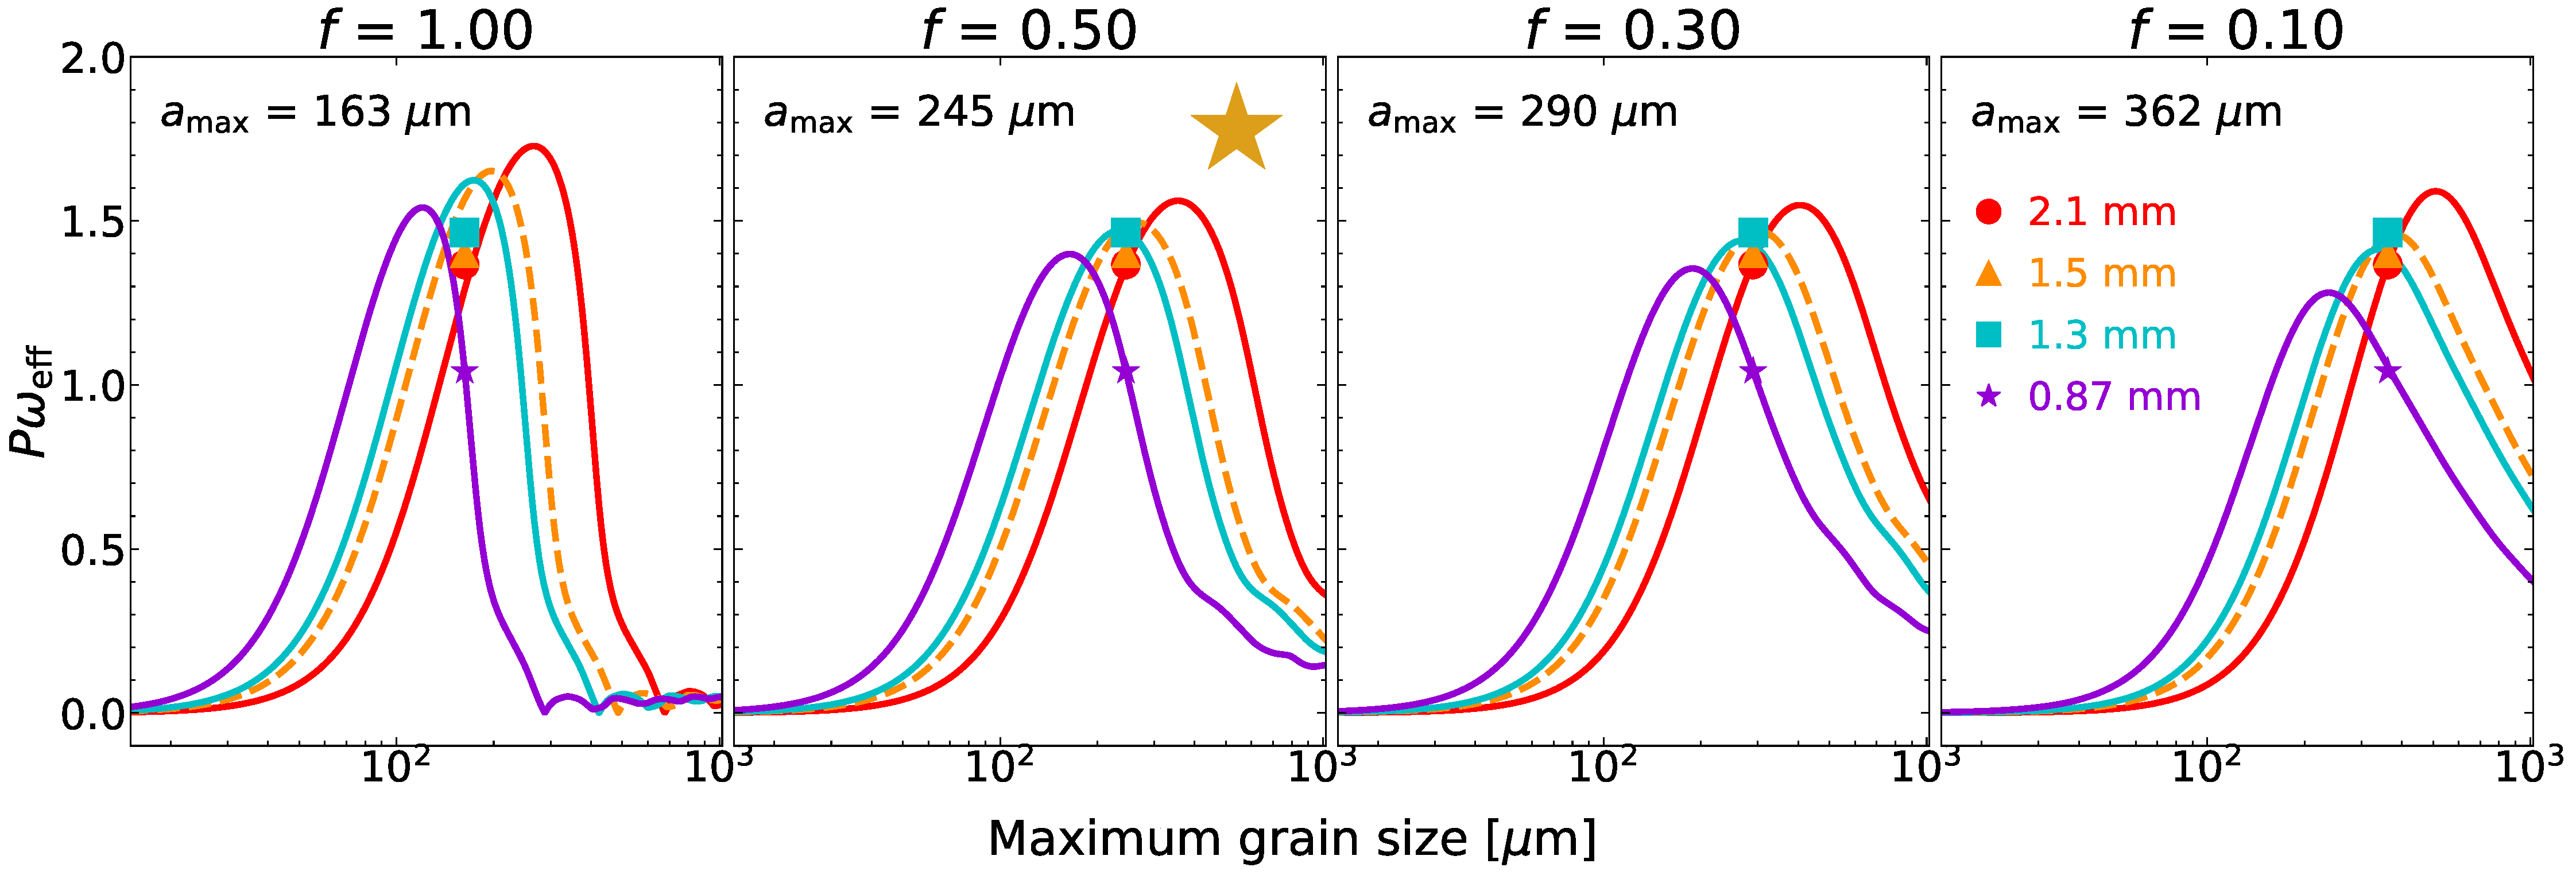
\includegraphics[width=0.99\textwidth]{WRITEUP_AND_IMAGES/IMAGES/WRITEUP/DustModels/DustModelPlot_Without5_ZhangMethod.pdf}
  \caption[Curves of \Pweff multiplied by best-fit SF to compare to \POLFsiNS.]{Curves of \Pweff multiplied by best-fit SF (Equation \ref{eq: sf}) to compare to \POLFsiNS. Markers are \POLFsiNS, listed in Table \ref{tab: polf_comparison}. The best-fit (lowest $\chi^2$, Equation \ref{eq: chi_squared_dust_model}) is represented with a gold star. The specific results of the fit can be found in Table \ref{tab: dust_model_fits_spherical}. Wavelengths that are not included in the fit for the SF have a dashed line. \reduced{update this after reduced chi squared}}
  \label{fig: Spherical_BEST}
\end{figure}


% ----------------------------------------------



% ----------------------------------------------------------------
\begin{figure}[htbp]
  \centering
  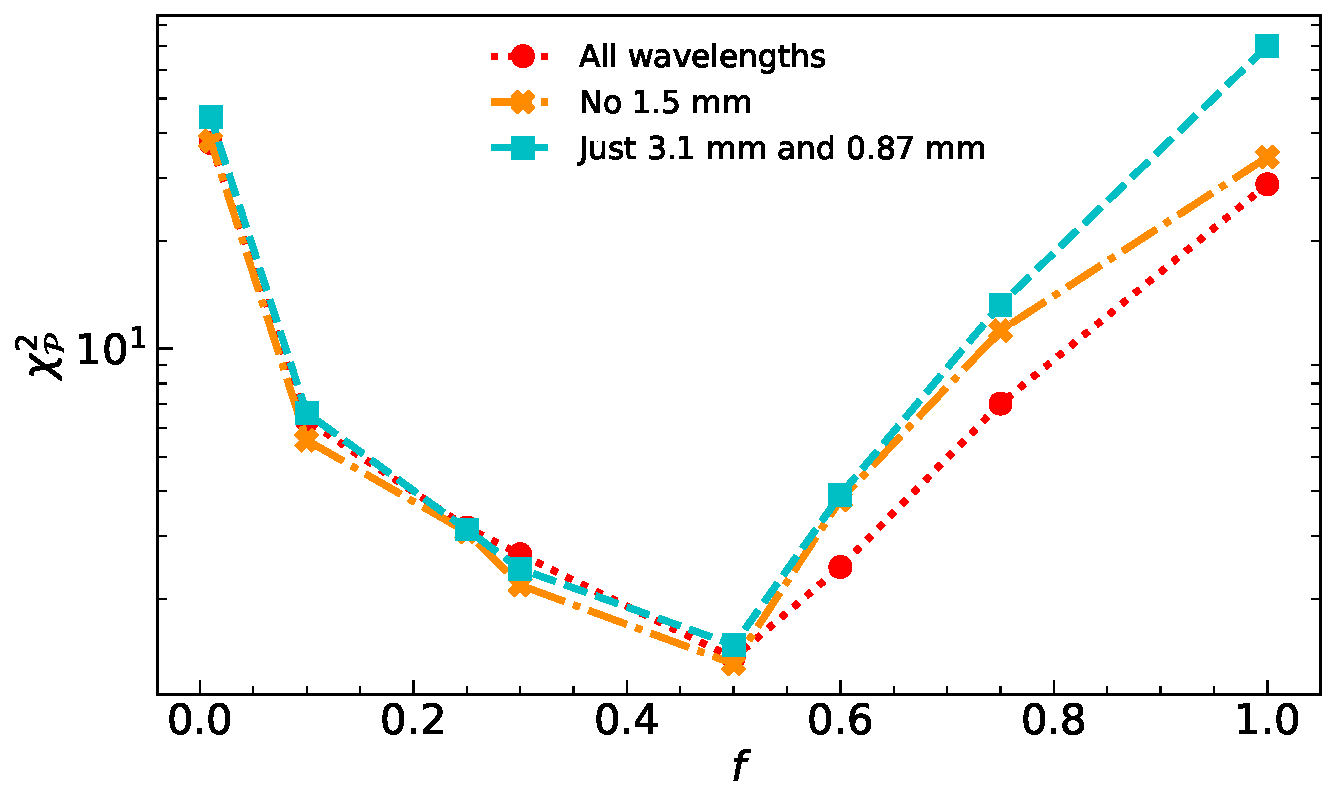
\includegraphics[width=0.75\textwidth]{WRITEUP_AND_IMAGES/IMAGES/WRITEUP/DustModels/chi_fs_f.pdf}
  \caption[Plot of filling factor, $f$, versus the goodness-of-fit parameter, $\chi_\mathcal{P}^2$.]{Plot of filling factor, $f$, versus the goodness-of-fit parameter, $\chi_\mathcal{P}^2$, showing a local minimum at $f = 0.5$ for all fitting cases for spherical grains. \reduced{update this after reduced chi squared}} 
  \label{fig: chi_vs_f}
\end{figure}
% ----------------------------------------------------------------
\subsection{Irregular Dust Models}

Table \ref{tab: dust_model_fits_irregular} reports the results of the irregular grain fits. Figure \ref{fig: irregular_fits} shows the results of these fits. The lowest $\chi_\mathcal{P}^2$ occurs for the all-wavelengths case with a best-fit grain size of \ibestNS. 

% ------------------------------------------------------
\begin{table}[h!]
\centering
\caption{Same as Table \ref{tab: dust_model_fits_spherical} but for irregular grains. \reduced{update this after reduced chi squared}}
\begin{tabular}{lccc}
\toprule
\textbf{Fit Case} &  \textbf{Scale Factor (SF)} & $\boldsymbol{\chi_\mathcal{P}^2}$ & \textbf{$\boldsymbol{\amaxEQ}$ ($\boldsymbol{\mu}$m)} \\
\midrule

All wavelengths  & \textbf{1.83} & \textbf{4.54} & \textbf{209} \\
No \bfive               & 1.88 & 5.93 & 211 \\
Just \bfour and \bseven & 1.90 & 8.71 & 212 \\
\bottomrule
\end{tabular}
\label{tab: dust_model_fits_irregular}
\end{table}
% ------------------------------------------------------

% ----------------------------------------------


% ----------------------------------------------------------------
\begin{figure}[htbp]
  \centering
  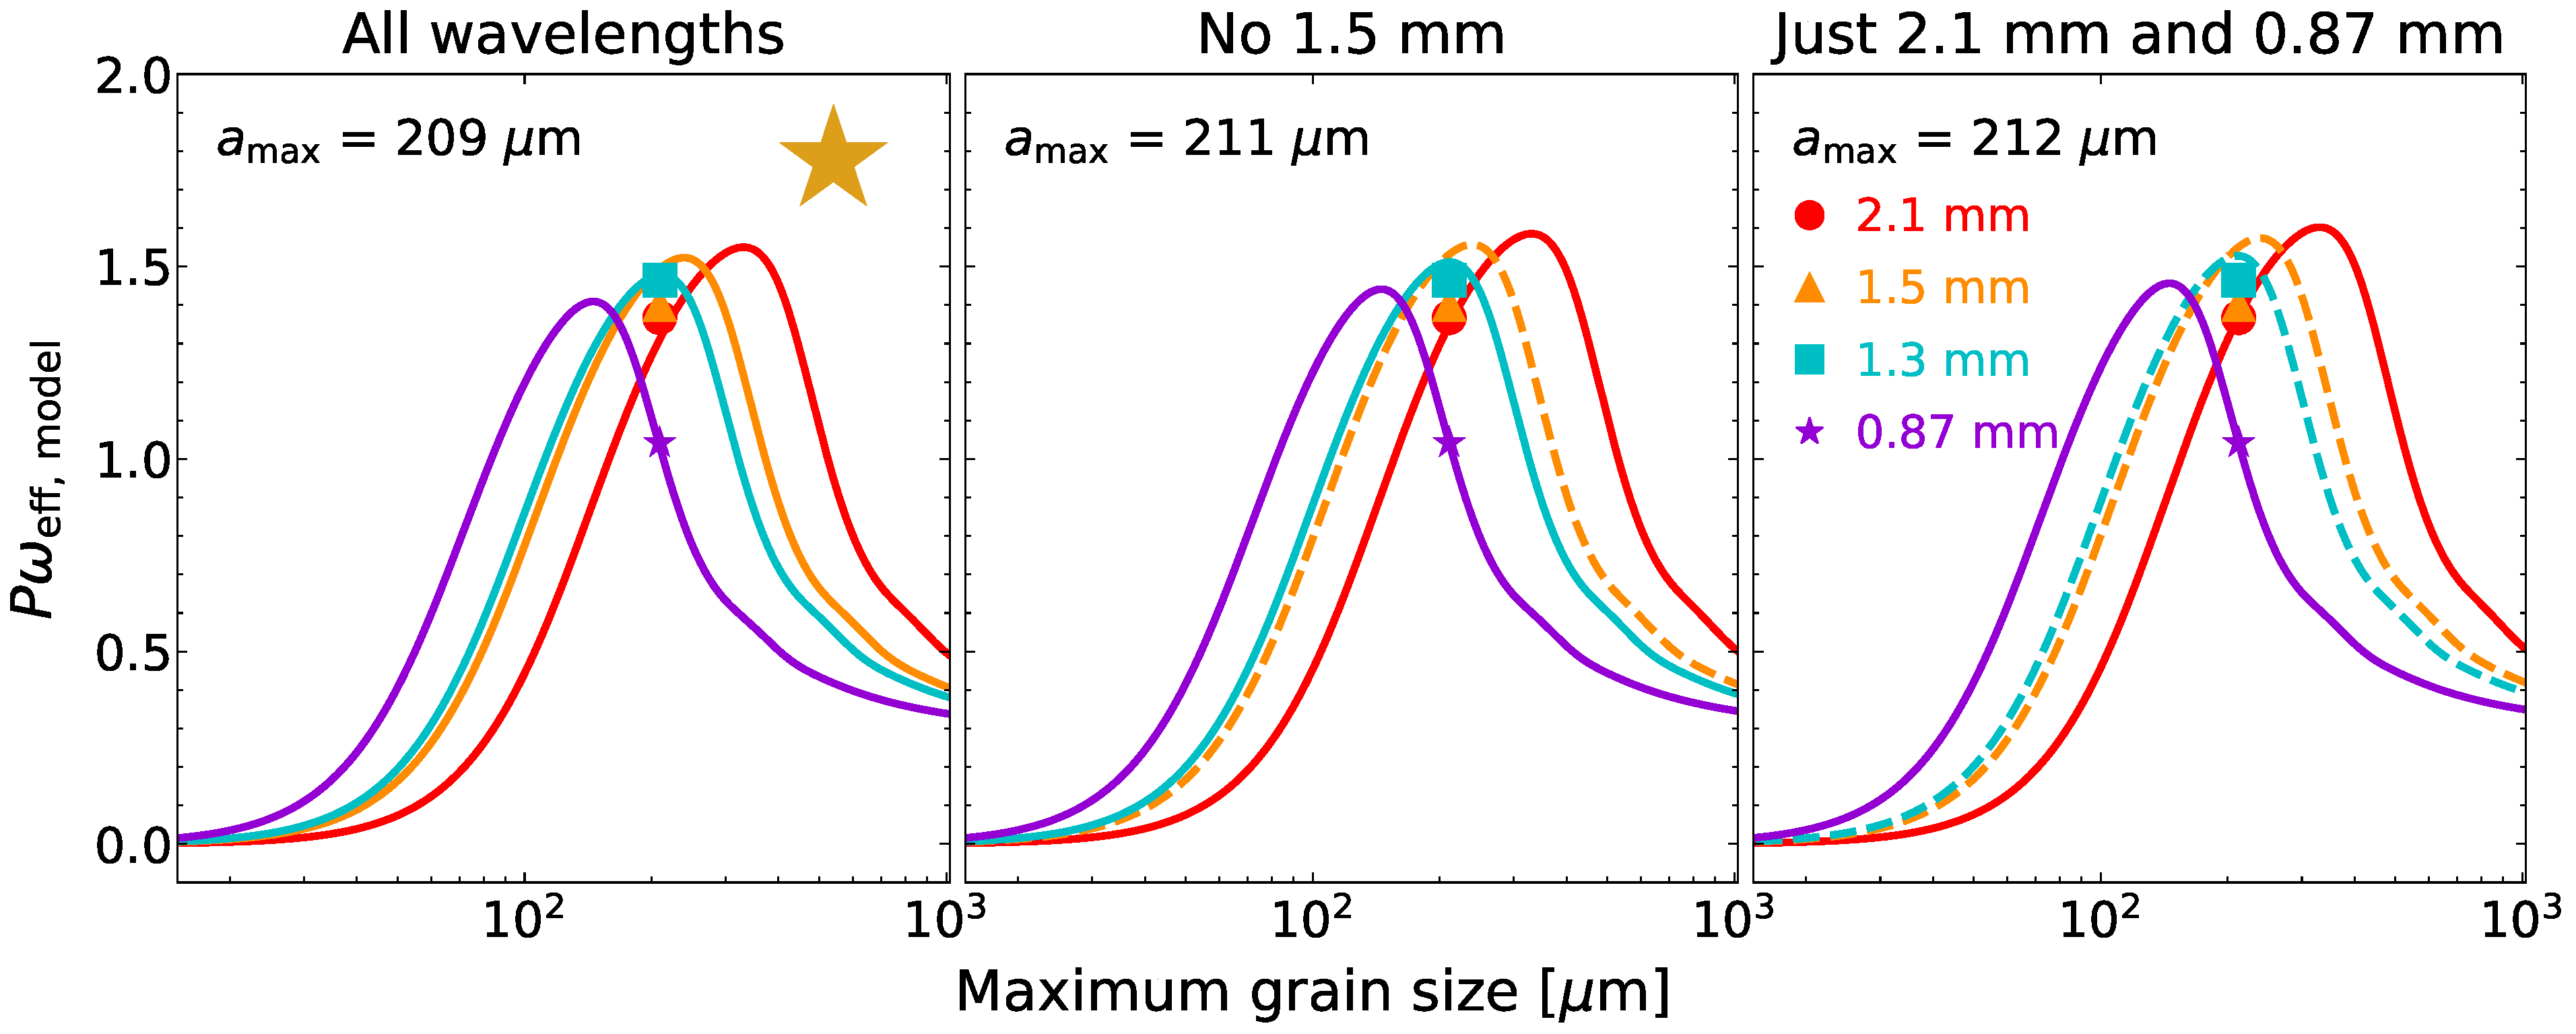
\includegraphics[width=0.99\textwidth]{WRITEUP_AND_IMAGES/IMAGES/WRITEUP/glitterin/DustModelPlot_GlitterinGrid_only3_omega_eff.pdf}
  \caption[Same as Figure \ref{fig: Spherical_BEST} but for irregular dust grains.]{Same as Figure \ref{fig: Spherical_BEST} but for irregular dust grains. Porosity is fixed, and the grid shows the results for each fitting case. Corresponding results can be found in Table \ref{tab: dust_model_fits_irregular}.  \reduced{update this after reduced chi squared}} 
  \label{fig: irregular_fits}
\end{figure}
% ----------------------------------------------------------------